\documentclass[11pt,a4paper]{article}

\usepackage[T1]{fontenc}
\usepackage[utf8]{inputenc}
\usepackage[spanish,es-noshorthands,es-tabla]{babel}
\usepackage{lmodern}
\usepackage{microtype}
\usepackage[margin=2.4cm]{geometry}
\usepackage{xcolor}
\usepackage{booktabs}
\usepackage{tabularx}
\usepackage{array}
\usepackage{enumitem}
\usepackage{caption}
\usepackage{fancyvrb}
\usepackage{graphicx}
\graphicspath{{../capturas/}}
\usepackage{tikz}
\usetikzlibrary{arrows.meta}
\usepackage[hidelinks]{hyperref}

\definecolor{tcpc}{RGB}{105,75,170}
\definecolor{udpc}{RGB}{25,105,175}

\newcommand{\code}[1]{\texttt{#1}}
\newcommand{\crlf}{\texttt{\textbackslash r\textbackslash n}}
% Recuadro rojo para lo que falta antes de entregar. Para ocultarlos todos de una vez:
% \renewcommand{\pendiente}[1]{}
\newcommand{\pendiente}[1]{\par\smallskip\noindent\fcolorbox{red!70!black}{red!4}{%
  \parbox{\dimexpr\linewidth-2\fboxsep-2\fboxrule}{\small\textbf{Pendiente.} #1}}\par\smallskip}

\setlist{itemsep=2pt,topsep=4pt}
\captionsetup{font=small,labelfont=bf}
\setlength{\parskip}{4pt}
\setlength{\emergencystretch}{2em}

\title{\textbf{TPD: Desarrollo de aplicaciones distribuidas con BSD sockets}\\[4pt]
  \large i310 Redes y Comunicación - Universidad de San Andrés}
\author{Grupo 12 (usuario \code{grupo12})\\[2pt]
  Martín De Hie \quad Sol García Pereyra \quad Máximo Barral}
\date{Noviembre de 2026}

\begin{document}
\maketitle

\section{Introducción}

El trabajo consiste en un cliente escrito en C con la biblioteca BSD sockets que resuelve dos desafíos contra el
servidor de la cátedra. En el primero, el cliente averigua su IP pública con un pedido HTTP escrito a mano, se
autentica por UDP con una firma MD5 y obtiene un puerto TCP abierto dinámicamente. En el segundo, se conecta a ese
puerto, separa las unidades de datos de protocolo (PDUs, por \textit{Protocol Data Units}) que llegan por el stream
TCP, valida cada una y la reenvía firmada por UDP junto con su código de parseo.

En este informe vamos a describir primero la estructura del cliente y cómo resuelve cada desafío. Después, se presentarán las pruebas, las capturas y las respuestas a las cuatro preguntas.
Las instrucciones de compilación y uso están en el \code{README.md} del repositorio.

\section{Estructura del cliente}

El código del TP completo está en \code{src/} y se divide en nueve módulos (Tabla~\ref{tab:modulos}). Ninguno usa
bibliotecas externas, como pide la consigna: el HTTP está implementado sobre la biblioteca estándar y los sockets, y
el MD5 es la implementación en C que la cátedra brindó como código de ayuda. Del mismo código de ayuda tomamos dos
funciones para el primer desafío, \code{skip\_single} y \code{timeval\_subtract} (Sección~\ref{sec:auth}). La
descripción de cada función pública está en su correspondiente \code{.h}. La Figura~\ref{fig:secuencia} muestra el recorrido
completo de los mensajes.

\begin{table}[h]
\centering\small
\begin{tabularx}{\linewidth}{@{}l X@{}}
\toprule
Archivo & Responsabilidad \\
\midrule
\code{main.c} & Encadena los pasos: credenciales, IP pública, autenticación y reenvío. \\
\code{credentials.c} & Lee y valida el archivo de credenciales (IP del servidor, usuario y secreto). \\
\code{auth.c} & Primer desafío: pide el puerto TCP por UDP y verifica la firma de la respuesta. Incluye \code{skip\_single} y \code{timeval\_subtract} del código de ayuda de la cátedra. \\
\code{forward.c} & Segundo desafío: recibe el stream TCP, delimita y valida cada PDU y la reenvía firmada por UDP. \\
\code{http\_ip.c} & Obtiene la IP pública con un \code{GET / HTTP/1.0} a \code{api.ipify.org} sobre un socket TCP. \\
\code{md5.c} & Implementación de MD5 del código de ayuda de la cátedra, sin modificaciones. Devuelve los 16 bytes del digesto. \\
\code{md5\_hex.c} & Calcula el MD5 con \code{md5.c} y lo convierte en los 32 caracteres hexadecimales en minúscula que usan las firmas. \\
\code{framing.c} & Acumula los bytes del stream TCP y extrae las PDUs completas, delimitadas por \crlf. \\
\code{pdu.c} & Valida una PDU ya delimitada y devuelve su código de parseo (200, 400 o 405 a 410). \\
\bottomrule
\end{tabularx}
\caption{Módulos del cliente.}
\label{tab:modulos}
\end{table}

\begin{figure}[h]
\centering
\begin{tikzpicture}[x=1cm,y=-0.6cm,font=\small,
    msg/.style={-{Stealth[length=2mm]},thick},
    tcp/.style={msg,color=tcpc}, udp/.style={msg,color=udpc},
    lbl/.style={above,fill=white,inner sep=1pt,font=\footnotesize\ttfamily}]
  \foreach \x/\n in {0/Cliente, 3.9/api.ipify.org:80, 8/{Servidor UDP\\:20262}, 12.1/{Servidor TCP\\:30001}}{
    \node[draw,rounded corners=2pt,fill=gray!8,minimum width=2.7cm,minimum height=0.9cm,align=center] at (\x,0) {\n};
    \draw[dashed,gray] (\x,0.9) -- (\x,13.4);
  }
  \draw[tcp] (0,1.8) -- node[lbl]{GET / HTTP/1.0} (3.9,1.8);
  \draw[tcp] (3.9,2.9) -- node[lbl]{200 OK: 181.9.209.54} (0,2.9);
  \draw[udp] (0,4.3) -- node[lbl,pos=.45]{grupo12|181.9.209.54|firma} (8,4.3);
  \draw[udp] (8,5.4) -- node[lbl,pos=.55]{200|Port|30001|firma} (0,5.4);
  \draw[tcp] (0,6.8) -- node[lbl,pos=.8]{connect() antes de 10s} (12.1,6.8);
  \draw[gray,rounded corners=2pt] (-1.45,7.6) rectangle (13.55,11.4);
  \node[anchor=north west,font=\footnotesize\itshape,text=gray,fill=white,inner sep=1pt] at (-1.35,7.7) {mientras haya datos};
  \draw[tcp] (12.1,8.7) -- node[lbl,pos=.25]{PDU\textbackslash r\textbackslash n PDU\textbackslash r\textbackslash n ...} (0,8.7);
  \draw[udp] (0,10.2) -- node[lbl,pos=.5]{grupo12|PDU|código|firma} (8,10.2);
  \node[font=\footnotesize,text=gray,align=left,anchor=west] at (8.2,10.2) {una por cada PDU\\sin \code{|}};
  \draw[tcp] (12.1,12.5) -- node[lbl,pos=.25]{FIN} (0,12.5);
\end{tikzpicture}
\caption{Recorrido de los mensajes, con los valores de una corrida del checkpoint. En violeta va lo que viaja por TCP
y en azul lo que viaja por UDP. La firma es el MD5 del mismo mensaje con el secreto en lugar de la firma, de modo
que el secreto nunca viaja por la red.}
\label{fig:secuencia}
\end{figure}

\section{Primer desafío: autenticación}
\label{sec:auth}

\textbf{IP pública.} El servidor valida la IP que el cliente declara en el mensaje, y esa IP no es la de la
interfaz de la máquina. En la corrida del checkpoint, el paquete salió de \code{172.20.10.2}, una dirección privada, y el servidor lo vio llegar desde \code{181.9.209.54}: en el medio hay un NAT (traductor de direcciones
de red) que reescribe la dirección de origen. Por eso el cliente le pregunta su IP pública a \code{api.ipify.org}.

\textbf{Pedido HTTP.} El pedido es un \code{GET / HTTP/1.0} escrito a mano sobre un socket TCP. Usamos HTTP/1.0 y
no 1.1 porque así el servidor cierra la conexión al terminar la respuesta, y ese cierre marca dónde termina sin tener
que interpretar \code{Content-Length} ni \textit{chunked encoding}. Como TCP puede entregar la respuesta repartida
en varios \code{recv}, el cliente lee hasta que \code{recv} devuelve 0. Después busca el cuerpo a continuación de
la línea vacía (\code{\textbackslash r\textbackslash n\textbackslash r\textbackslash n}) y verifica con
\code{inet\_pton} que sea una IPv4.

\textbf{Firma.} El mensaje es \code{<USERNAME>|<IPv4ADDRESS>|<SIGNATURE>}, donde la firma es el MD5 en hexadecimal
de \code{<USERNAME>|<IPv4ADDRESS>|<SECRET>}. El secreto entra en el digesto pero nunca viaja, y el servidor, que
también lo conoce, puede recalcular la firma y comprobar que el mensaje viene de quien dice. La respuesta se
verifica de la misma forma. La función \code{md5} de la cátedra calcula el digesto, devolviendo 16 bytes, y
\code{md5\_hex} los convierte en los 32 caracteres hexadecimales en minúscula.

\textbf{Espera de la respuesta.} Para lograr la espera de 10 segundos y descartar en silencio las respuestas mal
firmadas, un \code{SO\_RCVTIMEO} fijo de 10 segundos no alcanza: el timeout es por llamada, así que cada datagrama
inválido reiniciaría la espera y una sucesión de respuestas inválidas la extendería sin límite. Por eso la función
\code{autenticar} fija un \textbf{plazo absoluto}, el cual esta generado por la hora de \code{gettimeofday} más 10 segundos. Antes de cada
\code{recvfrom}, calcula con \code{timeval\_subtract}, tomada del código de ayuda de la cátedra, cuánto falta para ese
plazo y lo usa como timeout. Si la resta da negativa o exactamente cero, la espera terminó. El cero se trata aparte
porque un \code{SO\_RCVTIMEO} de 0 no significa ``no esperar'', sino esperar sin límite. Como \code{gettimeofday} da
la hora del sistema, un ajuste del reloj justo durante esos 10 segundos alargaría o acortaría la espera. Pero con un plazo
tan corto, no lo consideramos un problema.

\textbf{Verificación de la respuesta.} Cada respuesta pasa por \code{procesar\_respuesta}, que separa los cuatro
campos, verifica la firma y solo acepta \code{200|Port|<puerto>} con un puerto entre 1 y 65535. Los campos se
separan con \code{skip\_single}, del código de ayuda de la cátedra: corta en el primer pipe, lo reemplaza por
\code{'\textbackslash 0'} y avanza al campo siguiente. A diferencia de \code{strtok}, toma un solo delimitador por
vez, así que respeta los campos vacíos. Y en el caso de un pipe de más, este queda dentro de la firma y la invalida. Lo que
\code{skip\_single} no hace es avisar cuando no encuentra el pipe: en ese caso deja el puntero después del final del
string, y la lectura siguiente se sale del buffer. Por eso \code{procesar\_respuesta} primero cuenta que haya al
menos tres pipes y, si faltan, descarta la respuesta (Sección~\ref{sec:pruebas-catedra}). Con los campos ya
separados, la firma esperada es el MD5 de \code{<CODE>|<ACTION>|<TEXT>|<SECRET>}. Una respuesta \code{4xx} con la
firma de 32 ceros se informa como error y termina el programa. Cualquier otra respuesta se descarta.

\section{Segundo desafío: framing, validación y reenvío}

\subsection{Framing}

TCP entrega un \textbf{stream de bytes, no mensajes}: un \code{recv} puede traer media PDU, varias, o una cantidad no
entera de ellas, que son los tres casos de ``Pruebas a superar''. Por eso el cliente no interpreta lo
que devuelve cada \code{recv}, sino que lo acumula en un \code{struct framer} con un buffer de 4096 bytes
(\code{FRAMER\_CAPACIDAD}). Después de cada \code{recv}, un bucle llama a \code{framer\_siguiente} hasta que no quedan
PDUs completas. Esa función busca el primer \crlf{} en todo lo acumulado y no solo en los bytes nuevos, porque el
\code{\textbackslash r} puede llegar al final de un \code{recv} y el \code{\textbackslash n} al principio del
siguiente. Cuando lo encuentra, copia la PDU sin el delimitador y corre el resto al principio del buffer con
\code{memmove}. No se usa \code{strstr} porque el buffer no termina en \code{'\textbackslash 0'} y puede contener
ese byte.

Además, quedan otros dos casos borde: si se acumulan 4096 bytes sin un solo \crlf, eso no puede ser una PDU (el máximo es de 122
bytes), así que se descarta y se sigue con lo nuevo. Y si el servidor cierra la conexión con bytes sin delimitar en el
buffer, esos bytes no se reenvían, porque la consigna pide reenviar solo las PDUs delimitadas.

\subsection{Validación}

La función \code{validar\_pdu(pdu, len, hora\_actual)} recibe la hora actual como parámetro. Eso permite probarla de
forma determinista con el ``timestamp actual'' de los ejemplos de la consigna (\code{1792303547}), mientras que el
cliente le pasa \code{time(NULL)}. También recibe el largo explícito, porque una PDU inválida puede traer un byte
\code{0x00} que tiene que contar como carácter inválido y no cortar la PDU.

Los siete ejemplos de la consigna fijan el resultado de los casos típicos, pero no la precedencia entre errores ni
algunos bordes. La Tabla~\ref{tab:decisiones} resume lo que decidimos. Todas las decisiones son compatibles con los
siete ejemplos y están aisladas en \code{pdu.c}, así que cambiar una precedencia es intercambiar dos \code{if}.

\begin{table}[h]
\centering\small
\begin{tabularx}{\linewidth}{@{}>{\raggedright\arraybackslash}p{4.2cm} >{\raggedright\arraybackslash}p{2.1cm} X@{}}
\toprule
Caso & Decisión & Motivo \\
\midrule
Sin \code{\&} & 400 & Es el ejemplo de la consigna (``no hay 2 campos''). \\
Más de un \code{\&} & 408 & Se corta en el primero, y el \code{\&} está excluido de los caracteres del mensaje. \\
Timestamp vacío & 400 & No tiene caracteres inválidos (405) ni sobra largo (407): es un error no tipificado. \\
Precedencia en el timestamp & 405, 407, 406 & Si no son todos dígitos no es un número, y su largo no importa. Un número de más de 11 dígitos no se interpreta como hora. \\
300 s exactos de antigüedad & 200 & La consigna dice ``más de 300 segundos'', así que 300 todavía es válido. \\
Timestamp en el futuro & 200 & La consigna solo define el vencimiento por antigüedad. \\
Precedencia en el mensaje & 409, 410, 408 & Primero el tamaño del campo y después su contenido. \\
Byte \code{0x00} en el mensaje & 408 & Está fuera del rango 0x20--0x7D. \\
\bottomrule
\end{tabularx}
\caption{Decisiones de validación donde la consigna no es explícita.}
\label{tab:decisiones}
\end{table}

\subsection{Reenvío}

Cada PDU se reenvía como \code{<USERNAME>|<PDU>|<PARSE\_CODE>|<SIGNATURE>}, firmada sobre el mismo mensaje con el
secreto en lugar de la firma. Los dos strings se construyen con la función \code{armar}, que copia la PDU con
\code{memcpy} según su largo en lugar de usar \code{printf} con \code{\%s}. Las PDUs que contienen \code{|} no se
reenvían, porque romperían el formato del mensaje UDP. Se buscan con \code{memchr} y no con \code{strchr}, porque
\code{strchr} se detendría en un \code{0x00} anterior al pipe.

La primera versión de \code{reenviar\_pdu} tenía dos defectos que corregimos al revisarla:

\begin{enumerate}
\item Calculaba el largo con \code{strlen} y armaba el mensaje con \code{\%s}. Una PDU como
  \code{<t>\&ab\textbackslash 0c} (con un byte \code{0x00}) se validaba y se reenviaba truncada como
  \code{<t>\&ab}, con código 200 en lugar de 408. La prueba de punta a punta de la Sección~\ref{sec:e2e} lo pone en
  evidencia: con la versión original, ese reenvío es el único que falla.
\item Los buffers medían \code{FRAMER\_CAPACIDAD + 2 * MAX\_CAMPO}, es decir 4224 bytes. El peor caso que admite el
  código es de 4227: 63 caracteres de usuario, una PDU de 4094, tres pipes, tres dígitos de código, 63 de secreto y
  el \code{'\textbackslash 0'}. En ese caso \code{snprintf} trunca pero devuelve el largo que \emph{habría}
  escrito, y \code{sendto} leería 3 bytes por fuera del buffer. Con nuestras credenciales el caso no se alcanza,
  pero el buffer tiene que cubrir lo que acepta \code{leer\_credenciales}. Ahora mide
  \code{FRAMER\_CAPACIDAD + 3 * MAX\_CAMPO} (4288 bytes).
\end{enumerate}

\section{Pruebas}

Mientras desarrollábamos el cliente no teníamos acceso al servidor de la cátedra, así que lo probamos con programas
propios que no lo necesitan: pruebas unitarias y un servidor simulado. No forman parte de la entrega, que contiene
solo la implementación, pero los resultados respaldan las decisiones de este informe.

\subsection{Pruebas unitarias}

Probamos \code{validar\_pdu} con los siete ejemplos de la consigna y su timestamp actual, y con ocho casos borde: el
mensaje de 100 caracteres (200) y el de 101 (410); la antigüedad de 300s (200) y la de 301s (406); el timestamp
vacío (400); el \code{\&} dentro del mensaje (408); el carácter \code{\textasciitilde} (0x7E, 408), y el byte
\code{0x00} en el medio del mensaje (408).

Probamos el framer con los tres casos de framing de la consigna: una PDU partida en cuatro \code{recv}, con el
\code{\textbackslash r} y el \code{\textbackslash n} en llamadas distintas; tres PDUs en un solo \code{recv}, y
tres PDUs repartidas en tres \code{recv} con una cola de 6 bytes sin delimitar, que debe quedar en el buffer. En los
dos módulos, todos los casos dieron el resultado esperado.

\subsection{Prueba de punta a punta con un servidor simulado}
\label{sec:e2e}

Como no teníamos acceso al servidor de la cátedra, escribimos con asistencia de inteligencia artificial un servidor
simulado en Python, para poder probar el cliente completo y avanzar con el desarrollo. Imita al servidor de la
cátedra en \code{127.0.0.1} con las credenciales de ejemplo de la consigna (\code{grupo01}, \code{secreto01}). Verifica la firma de la autenticación y responde primero con una firma inválida, que el cliente
tiene que ignorar, y después con el puerto bien firmado. Luego manda por TCP una PDU de cada código y una cola sin
delimitar, cortando el stream cada 37 bytes con \code{TCP\_NODELAY}, para que haya PDUs partidas y varias por
segmento. Al final, verifica la PDU, el código y la firma de cada reenvío. La Tabla~\ref{tab:e2e} muestra el
resultado de la versión final del cliente y el de la versión con el \code{reenviar\_pdu} original. En ambos casos
\code{validar\_pdu} es la implementación final.

\begin{table}[h]
\centering\small
\begin{tabular}{@{}l c c c@{}}
\toprule
PDU enviada (\code{<t>} es la hora actual) & Esperado & Versión final & \code{reenviar\_pdu} original \\
\midrule
\code{<t>\&Temperatura ambiente 11 grados} & 200 & 200 & 200 \\
\code{12345.1\&x} & 405 & 405 & 405 \\
\code{<t-1000>\&viejo} & 406 & 406 & 406 \\
\code{1111762303544\&y} & 407 & 407 & 407 \\
\code{<t>\&11 \textsuperscript{0}C} & 408 & 408 & 408 \\
\code{<t>\&} & 409 & 409 & 409 \\
\code{<t>\&a\ldots a} (101 caracteres) & 410 & 410 & 410 \\
\code{<t>\textasciicircum z} & 400 & 400 & 400 \\
\code{<t>\&C|pipe} & no se reenvía & no se reenvía & no se reenvía \\
\code{<t>\&ab\textbackslash 0c} & 408 & 408 & \textbf{200, PDU truncada} \\
\midrule
Reenvíos correctos & & \textbf{9/9} & 8/9 \\
\bottomrule
\end{tabular}
\caption{Prueba de punta a punta contra el servidor simulado. La firma inválida de la autenticación se
descartó en las dos corridas, y los 20 bytes finales sin delimitar no se reenviaron.}
\label{tab:e2e}
\end{table}

El servidor simulado implementa \textbf{nuestra lectura} de la consigna, así que no puede detectar una
interpretación distinta de la de la cátedra: valida que el cliente hace lo que decidimos, no que lo decidido coincida
con lo que espera la cátedra. Eso solo lo confirma la corrida contra el servidor de la cátedra
(Sección~\ref{sec:capturas}).

\subsection{Pruebas del cambio al código de ayuda de la cátedra}
\label{sec:pruebas-catedra}

Cuando la cátedra brindó su código de ayuda, reemplazamos por él las partes del primer desafío que habíamos resuelto
con código propio: el MD5, la separación de los campos de la respuesta y el cálculo del tiempo que falta para el
plazo. El segundo desafío no cambió. Para verificar el reemplazo escribimos, también con asistencia de inteligencia
artificial, las pruebas de la Tabla~\ref{tab:catedra}, que no necesitan el servidor de la cátedra.

\begin{table}[h]
\centering\small
\begin{tabularx}{\linewidth}{@{}>{\raggedright\arraybackslash}p{3.4cm} >{\raggedright\arraybackslash}X c@{}}
\toprule
Qué se probó & Casos & Resultado \\
\midrule
MD5 & El MD5 de la cátedra contra nuestra implementación anterior y contra \code{hashlib} de Python: los dos ejemplos
  de la consigna, el del código de ayuda y mensajes de todos los largos entre 0 y 200 bytes, que incluyen los bordes
  del relleno (55, 56 y 64 bytes). & 204/204 \\
\code{procesar\_respuesta} & La respuesta del ejemplo de la consigna; puertos 1 y 65535; errores 400 y 401 firmados
  con ceros y un 401 con otra firma; firma alterada; puertos 0, 65536, vacío y con letras; código o acción
  distintos; un campo de más; respuestas sin uno, dos o los tres pipes; solo pipes, y la respuesta vacía. & 19/19 \\
\code{autenticar} & Contra un servidor UDP simulado en \code{127.0.0.1}, que además verifica que el pedido sea el del
  ejemplo de la consigna: respuesta válida; basura y respuestas mal firmadas antes de la válida; error 401; sin
  respuesta, y respuestas mal firmadas a los 3 y a los 6 segundos. En los dos últimos casos el cliente terminó a los
  10,05 s: el plazo es total y no se reinicia con cada datagrama. & 5/5 \\
\bottomrule
\end{tabularx}
\caption{Pruebas del primer desafío después de pasar al código de ayuda de la cátedra.}
\label{tab:catedra}
\end{table}

Las pruebas de \code{procesar\_respuesta} se compilaron con AddressSanitizer, y cada respuesta se copió a un buffer
del tamaño justo para que cualquier lectura por fuera del string quede en evidencia. Así comprobamos que el conteo de
pipes es necesario: si se lo quita, las respuestas a las que les falta algún pipe hacen que se lea fuera del buffer,
y AddressSanitizer lo reporta.

Por último, corrimos el cliente contra el servidor de la cátedra. Se autenticó, recibió el puerto 30075 y procesó
las 10 PDUs con los mismos resultados que en la corrida de la Sección~\ref{sec:capturas}.

\section{Capturas}
\label{sec:capturas}

La captura del TP completo está en \code{capturas/Final.pcapng}. La tomamos con Wireshark, capturando en todas las interfaces
con el filtro \code{host 167.114.129.206} para dejar afuera el resto del tráfico. Es de una corrida anterior al
cambio al código de ayuda de la cátedra (Sección~\ref{sec:pruebas-catedra}), pero el cambio no altera los bytes que
envía el cliente: con los mismos datos, el MD5 de la cátedra da las mismas firmas que el nuestro.

Desde la red Wi-Fi de la universidad el servidor no respondía la autenticación, probablemente por los filtros de
tráfico que menciona la consigna, así que la corrida final salió por una VPN (Tailscale). Por eso el cliente aparece
con la dirección \code{100.84.56.0}, aunque el servidor ve otra IP pública: es el mismo efecto del NAT descripto en la
Sección~\ref{sec:auth}.

\begin{figure}[h]
\centering
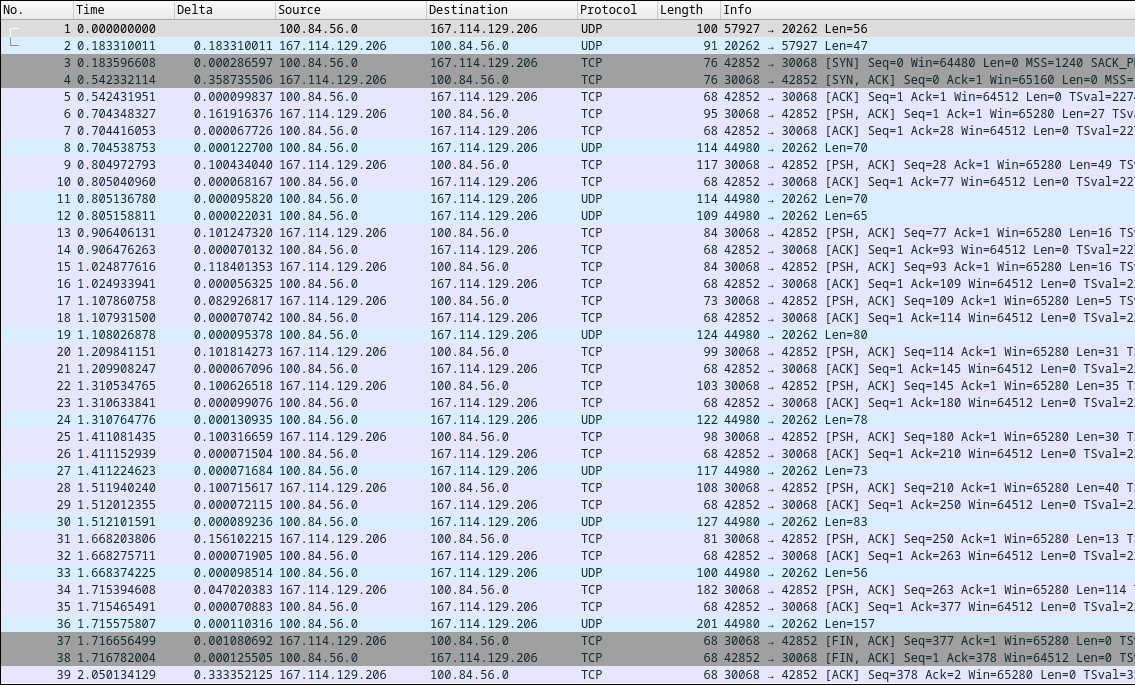
\includegraphics[width=\linewidth]{wireshark_paquetes.png}
\caption{Captura completa en Wireshark. En celeste, los datagramas UDP (autenticación y reenvíos); en lila, los
segmentos TCP; en gris, el SYN y los FIN.}
\label{fig:wireshark}
\end{figure}

En la Figura~\ref{fig:wireshark}, los paquetes 1 y 2 son la autenticación y la respuesta con el puerto 30068, y los
paquetes 3 a 5 son el \textit{three-way handshake}. Después llegan las PDUs por TCP, cada una seguida de su reenvío
por UDP, y la conexión se cierra con los FIN de los paquetes 37 y 38. La captura muestra dos de los casos de framing
de ``Pruebas a superar'': el segmento 9 trae dos PDUs completas, y la cuarta PDU llega partida en tres segmentos.

\begin{figure}[h]
\centering
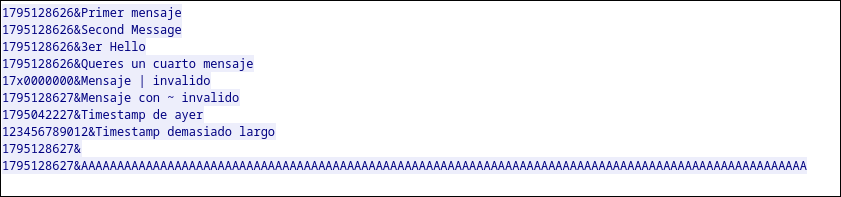
\includegraphics[width=0.85\linewidth]{wireshark_flujo_tcp.png}
\caption{Flujo TCP en Wireshark (\textit{Seguir} $\rightarrow$ \textit{Flujo TCP}): las 10 PDUs que envió el
servidor.}
\label{fig:flujo}
\end{figure}

El servidor envió 10 PDUs (Figura~\ref{fig:flujo}). El cliente reenvió nueve: cuatro con código 200 y el resto con
408, 406, 407, 409 y 410. La quinta contiene un pipe y no se reenvió. El servidor no responde a los reenvíos, así que
el cliente no puede saber si llegaron (Pregunta~3).

\section{Respuestas a las preguntas}

\subsection*{1. ¿Cómo podría mejorar el protocolo para permitir el reenvío de PDUs con el carácter 0x7C?}

Hoy el cliente no reenvía las PDUs que contienen \code{|}, así que el servidor se queda sin su código de parseo. El problema de fondo es que el mismo byte cumple dos funciones: es dato dentro de
la PDU y separador entre los campos del datagrama. Vemos cuatro formas de resolverlo, ordenadas de menor a mayor
cambio en el formato.

\textbf{Parseo posicional, sin cambiar el formato:} El usuario solo admite \code{[0-9A-Za-z]}, el código de parseo
tiene tres dígitos y la firma 32 caracteres hexadecimales, así que ninguno de esos campos puede contener un pipe.
Por lo tanto, el datagrama deja de ser ambiguo si el receptor corta en el primer pipe y en los dos últimos, y toma
todo lo que queda en el medio como la PDU. Así parsea los reenvíos nuestro servidor simulado
(\code{split(b"|", 1)} y \code{rsplit(b"|", 2)}). No agrega un solo byte, pero solo funciona mientras el mensaje
tenga un único campo libre: si el protocolo sumara otro, la ambigüedad volvería. Es una propiedad del formato
actual, no un mecanismo.

\textbf{Byte stuffing:} Es la solución de PPP: un byte de escape, 0x7D, indica que el byte siguiente
es especial y viaja con un XOR 0x20. Aplicado acá, el pipe (0x7C) se enviaría como \code{0x7D 0x5C} y el escape mismo
(\code{\}}, 0x7D) como \code{0x7D 0x5D}. Este último también hay que escaparlo, porque 0x7D es justo el límite
superior del rango permitido en el mensaje. El costo es un byte por cada aparición, de modo que en el peor caso la
PDU se duplica (de 122 a 244 bytes).

\textbf{Prefijo de longitud:} El mensaje pasaría a ser
\begin{center}\code{<USERNAME>|<LARGO>|<PDU>|<PARSE\_CODE>|<SIGNATURE>}\end{center}
y el receptor leería \code{LARGO} bytes sin mirar su contenido, como hace HTTP con \code{Content-Length}. El costo es fijo: para una PDU de hasta 122 bytes son a lo sumo
4 bytes (\code{|122}). Además acepta cualquier byte, incluido el \code{0x00} que, como se vio en la
Sección~\ref{sec:e2e}, puede aparecer en una PDU inválida.

\textbf{Codificación de la PDU.} Consiste en convertir la PDU a un alfabeto sin pipe. Base64 convierte 122 bytes en 164, un 34\,\% más, y
hexadecimal en 244. El \textit{percent-encoding} de las URLs solo reemplaza el pipe por \code{\%7C} y el
\code{\%} por \code{\%25}, a 3 bytes por aparición, y deja la PDU legible en Wireshark.

Nos inclinamos por el \textbf{prefijo de longitud}: tiene un costo fijo y chico, no transforma la PDU y admite
cualquier byte. Además, es la alternativa clásica al uso de delimitadores, así que la misma idea habría evitado el
problema del framing por \crlf{} en TCP.

Con cualquiera de las cuatro opciones, el protocolo tiene que especificar si el MD5 se calcula sobre los bytes
transmitidos o sobre la PDU original. Recomendamos los transmitidos, así el servidor verifica la firma antes de
decodificar nada que haya llegado de la red.

\subsection*{2. ¿Podría el servidor iniciar la conexión TCP contra las computadoras de los alumnos?}

A nivel de sockets, sí. TCP no distingue entre cliente y servidor una vez establecida la conexión: la diferencia es
solo quién hace la apertura pasiva (\code{listen} y \code{accept}) y quién la activa (\code{connect}). Nuestro
programa tendría que crear un socket, hacer \code{bind} a un puerto, \code{listen} y \code{accept}, e informar ese
puerto en el mensaje de autenticación. El servidor ya conoce la IP pública, porque viaja en ese mismo mensaje.

En cambio, a nivel de red, no funcionaría para la mayoría de los grupos. Nuestra corrida del checkpoint lo muestra:
la máquina tenía la dirección privada \code{172.20.10.2} y el servidor la veía como \code{181.9.209.54}. Un NAT crea
traducciones solo para los flujos que salen de la red interna, así que un SYN entrante dirigido a
\code{181.9.209.54} no encuentra ninguna traducción y el NAT lo descarta, porque no sabe a qué máquina entregarlo.

Las formas de atravesar el NAT tampoco son prácticas. Abrir un puerto en el router (\textit{port forwarding}) es
imposible en la red de la universidad o en un hotspot del celular, y con un NAT de proveedor (CGNAT) ni
siquiera la IP pública del router pertenece al usuario. La traducción UDP que creó la autenticación no sirve, porque
es de otro protocolo y otro puerto, y las técnicas de \textit{hole punching} para TCP dependen del comportamiento de
cada NAT y no son confiables. A esto se suman los firewalls de los equipos y los filtros de tráfico de las
redes académicas, que la propia consigna menciona.

Hoy en día, el problema ya se logró resolver: en el modo activo de FTP, el cliente
anuncia un puerto con el comando \code{PORT} y el servidor abre la conexión de datos hacia él. Ese modo dejó de
funcionar detrás de firewalls y NATs, y por eso se generalizó el modo pasivo (\code{PASV}), en el que el
servidor abre un puerto, lo informa y el cliente se conecta. Es exactamente el diseño de este TP:
\code{200|Port|30001} cumple el papel de la respuesta \code{227 Entering Passive Mode}.

Invertir los roles tendría además un costo de seguridad. Un servidor que se conecta a la IP y el puerto que le indica
un mensaje puede usarse para conectarse a terceros, como en el \textit{FTP bounce attack}. La firma
limitaría esa posibilidad a los grupos autenticados, pero no la eliminaría.

En resumen, \textbf{el rol se puede invertir en el código, pero no en la red}.

\subsection*{3. ¿Cómo se vería afectado el funcionamiento de los desafíos ante la pérdida de paquetes?}

La respuesta depende de qué transporte usa cada etapa: TCP recupera las pérdidas a costa de demora, y UDP no las
recupera. La Tabla~\ref{tab:perdidas} resume el efecto sobre nuestro cliente.

\begin{table}[h]
\centering\small
\begin{tabularx}{\linewidth}{@{}>{\raggedright\arraybackslash}p{3.3cm} l X@{}}
\toprule
Etapa & Transporte & Efecto de una pérdida en nuestro cliente \\
\midrule
IP pública (ipify) & TCP & Solo demora, por las retransmisiones. El \code{connect} tiene un límite de 5s y los SYN salen en 0, 1 y 3s, así que se toleran dos SYN perdidos seguidos. \\
Autenticación & UDP & Si se pierde el pedido o la respuesta, el cliente espera los 10s completos y termina con \code{Timeout}. No hay reintento. \\
Conexión al puerto dinámico & TCP & El puerto escucha 10s. Los SYN salen en 0, 1, 3 y 7s, así que se toleran tres pérdidas seguidas. El siguiente saldría a los 15s, cuando el puerto ya cerró. \\
Recepción de PDUs & TCP & El stream llega completo y en orden, solo con demora. El framing no se ve afectado. Si una pausa supera los 10s de \code{SO\_RCVTIMEO}, se corta la recepción y se pierden las PDUs restantes. \\
Reenvío de PDUs & UDP & El datagrama se pierde sin aviso: el cliente no puede saberlo y el servidor recibe una PDU menos, así que el desafío falla. \\
\bottomrule
\end{tabularx}
\caption{Efecto de la pérdida de paquetes en cada etapa. Los tiempos de los SYN suponen un tiempo de retransmisión
(RTO) inicial de 1s que se duplica en cada intento, como hace Linux.}
\label{tab:perdidas}
\end{table}

En las etapas sobre TCP, la pérdida no rompe la lógica, solo la demora. Esto vale en particular para el framing:
como el \code{framer} trabaja sobre el stream de bytes y no sobre los segmentos, el reparto de los bytes entre
segmentos no lo afecta. Las retransmisiones incluso pueden cambiar los límites de los segmentos, porque un segmento
retransmitido puede llevar más datos que el original. Un cliente que supusiera una PDU por segmento fallaría
justamente en presencia de pérdidas.

Para que una pausa del stream supere nuestro timeout de 10s hacen falta varias pérdidas consecutivas del mismo
segmento. Con un RTO del orden de 0,4s (en la corrida del checkpoint, la autenticación tardó 216 ms en ir y volver,
y Linux suma un piso de 200 ms), la espera acumulada tras $k$ intentos fallidos es de aproximadamente
$0{,}4\,(2^k-1)$ segundos, y supera los 10 s recién con unas cinco pérdidas seguidas. Eso es más propio de un corte
de enlace que de una pérdida ocasional. Por la misma razón, la ventana de 300s del timestamp queda muy lejos de
cualquier demora por retransmisión.

En las etapas sobre UDP, la pérdida es definitiva. En la autenticación, el cliente nota la pérdida porque no llega
respuesta, pero no reintenta. Una mejora razonable sería retransmitir el pedido cada 2 o 3 segundos dentro de los
10s. Sería seguro, porque el cliente usa solo la primera respuesta válida, y el puerto extra que abriría el
servidor se cierra solo a los 10s.

El reenvío de PDUs es la etapa más frágil, porque ni siquiera hay una respuesta que falte: \textbf{las PDUs llegan
de forma confiable por TCP y salen de forma no confiable por UDP}. Mitigarlo exige cambiar el protocolo, por ejemplo
con un número de secuencia en cada reenvío y una confirmación (ACK) del servidor, lo que equivale a reconstruir sobre
UDP una parte de lo que TCP ya ofrece. UDP tampoco garantiza el orden ni evita los duplicados, así
que el número de secuencia también le serviría al servidor si espera los reenvíos en el orden del stream.

\subsection*{4. Dificultades, aprendizajes y consejos para futuros alumnos}

La primera dificultad conceptual es que TCP no entrega mensajes sino bytes. La tentación inicial es tratar
cada \code{recv} como una PDU, y el error no surge en una red local, donde cada envío del servidor suele
llegar en un solo \code{recv}. El caso más sutil es el del \crlf{} partido entre dos \code{recv}, que obliga a buscar el
delimitador en todo lo acumulado y no solo en lo nuevo. Este mismo problema reaparece al leer la respuesta HTTP de
ipify, que también puede llegar en varios pedazos.

La segunda es que en código de red un \code{char *} no es un string. Las funciones de C que paran en el
\code{'\textbackslash 0'} (\code{strlen}, \code{strchr}, \code{printf} con \code{\%s}) parecen funcionar hasta que
llega un byte \code{0x00}. Así fue como la primera versión del reenvío mandaba una PDU truncada con código 200, y lo
descubrimos recién cuando la prueba de punta a punta incluyó ese caso. La lección es llevar siempre el par
puntero y largo, y usar \code{memchr} y \code{memcpy}.

La tercera es dimensionar los buffers para el peor caso y no para el caso típico, y conocer bien las
funciones que se usan. \code{snprintf} protege el buffer, pero devuelve el largo que habría escrito, no el que
escribió, por lo que usarlo como largo para \code{sendto} convierte una truncación silenciosa en una lectura fuera del buffer.
Los timeouts tienen una sutileza parecida: \code{SO\_RCVTIMEO} limita cada llamada, no la espera total, y para
respetar los 10s de la consigna hubo que trabajar con un plazo absoluto.

La cuarta es que la red real no es la de la máquina: la IP de la interfaz no es la que ve el servidor, y
entender el NAT fue necesario tanto para el primer desafío como para responder la segunda pregunta.

Los consejos que dejaríamos a quienes programan con BSD sockets por primera vez son:
\begin{enumerate}
\item Compilar con \code{-Wall -Wextra} desde el primer día y no dejar pasar ningún warning.
\item Verificar el valor de retorno de cada llamada (\code{socket}, \code{connect}, \code{send}, \code{recv},
  \code{sendto}, \code{recvfrom}) y usar \code{perror}. Recordar que \code{send} puede enviar menos bytes de los
  pedidos y que \code{recv} devuelve 0 cuando el otro extremo cerró.
\item Trabajar siempre con un puntero y un largo para los datos que vienen de la red, nunca con \code{strlen}.
\item Probar cada pieza sin red antes de juntarlas: el MD5 contra el ejemplo de la consigna, el framing y la validación con pruebas unitarias, y el programa completo contra un servidor simulado en
  \code{127.0.0.1}. El servidor de la cátedra tiene ventanas de 10 s y no explica por qué rechaza algo.
\item Tener Wireshark abierto mientras se programa, con un filtro por la IP del servidor. Ver los bytes que
  realmente salen ahorra horas de suposiciones.
\item No olvidar \code{htons} y \code{ntohs} para los puertos, y leer las páginas del manual de las secciones 2 y 7
  (\code{man 2 recv}, \code{man 7 socket}, \code{man 7 tcp}) junto con la guía de Beej.
\end{enumerate}
\end{document}
